%%
%% $Id$
%%
%% Copyright (c) 2007-2008 Christian Fehler
%% Copyright (c) 2007-2008 Benjamin Mies
%%


\chapter{Perspektive}\label{Perspective}

In diesem Kapitel werden die Zukunftsperspektiven für das \gtitool besprochen.
Bei der Implementierung wurde besonderer Wert darauf gelegt, dass das \gtitool
leicht zu erweitern sein muss. Der dadurch entstandene Aufwand konnte dadurch
gerechtfertigt werden, dass Erweiterungen in der Zukunft leichter und somit
schneller integriert werden können.\vspace{10pt}


\section{Graphische Komponenten}\label{PerspectiveGraphics}

Wie in Abschnitt \ref{Graph} beschrieben verwenden wir zur graphischen
Darstellung der Automaten die Bibliothek JGraph. Diese Bibliothek bietet einen
sehr großen Funktionsumfang, der von uns nicht komplett ausgeschöpft werden
musste. Eine mögliche Implementierung für die Zukunft wäre es, diese Bibliothek
durch eine eigene Implementierung zu ersetzen, die dann nur den gewünschten
Umfang bietet und somit leichter zu warten und zu erweitern ist.\vspace{10pt}

Da eine solche Implementierung sehr viel Zeit in Anspruch nehmen würde, war es
uns im Rahmen der Diplomarbeit nicht möglich, neben den umgesetzten Komponenten
auch noch die graphischen Komponenten selbst zu implementieren. JGraph bot uns
die Möglichkeit sehr schnell und einfach bereits brauchbare Ergebnisse zu
erzielen. Es mussten einige in \ref{GraphJGraphAdaptation} beschriebene
Anpassungen vorgenommen werden, damit das Ergebnis unseren Vorstellungen
entsprach, aber diese waren im Gegensatz zu einer vollständigen Implementieren
zeitlich nicht so komplex.\vspace{10pt}

Zu einer möglichen Umsetzung ist zu sagen, dass sowohl Zustände wie auch
Übergänge implementiert werden müssen. Was gerade bei der Verwendung von parallel
Übergängen ein größeres Problem sein könnte, da dort die Übergänge nicht auf
einer Linie verlaufen. Der größte Nutzer bei einer eigenständigen Implementierung
wäre, das Änderungen leichter eingepflegt werden könnten, da dies bei der sehr
komplexen Implementierung von JGraph meistens problematisch war.\vspace{10pt}


\section{Reguläre Ausdrücke}

Die wohl wichtigste und komplexeste Erweiterung die für die Zukunft geplant
ist, ist die Unterstützung von regulären Ausdrücken. Der Benutzer soll somit in
der Lage sein, einen regulären Ausruck wie
(\Symbol{a}$\mid$\Symbol{b})*\Symbol{a}\Symbol{b}\Symbol{b} eingeben zu können.
Anschließend sollen im Idealfall mehrere Möglichkeiten bestehen, mit diesem
Ausdruck weiter zu arbeiten. Diese Möglichkeiten sollen nun kurz angesprochen
werden.\vspace{10pt}

%### removes texlipse warning
Der eingegebene reguläre Ausdruck soll mit dem in \cite[S.159ff]{Compilers}
beschriebenen McNaughton-Yamada-Thompson Algorithmus in einen Automaten
umgewandelt werden können. Diese Umwandlung sollte, wie die anderen Umwandlungen
auch, schrittweise durchgeführt werden. Dadurch soll es dem Benutzer ermöglicht
werden, den zur Umwandlung benutzten Algorithmus besser zu verstehen. Abbildung
\ref{FigureThompson} zeigt das Ergebnis, das bei einer solchen Umwandlung
entstehen würde.\vspace{10pt}
%### removes texlipse warning

\begin{figure}[h!]
\begin{center}
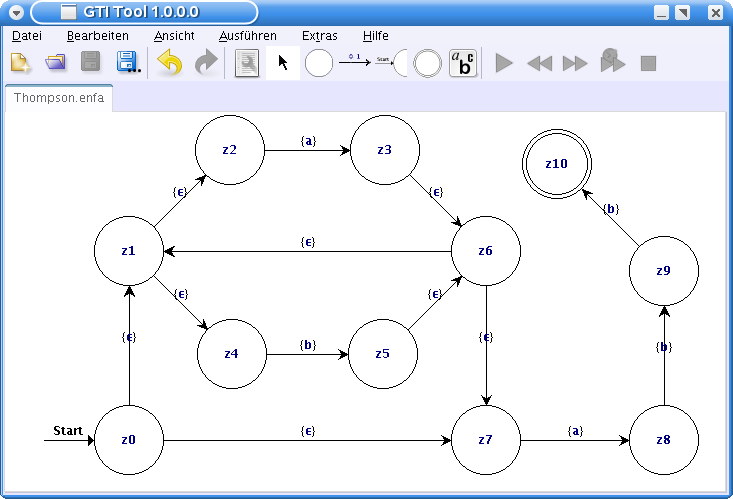
\includegraphics[width=12cm]{../images/thompson.png}
\caption{McNaughton-Yamada-Thompson Algorithmus}
\label{FigureThompson}
\end{center}
\end{figure}
\vspace{10pt}

%### removes texlipse warning
Eine weitere Verwendungsmöglichkeit eines regulären Ausdruck wäre das direkte
Umwandeln in einen DEA. Dieser Algorithmus wird in
\cite[S. 175ff]{Compilers} beschrieben und verwendet die Funktionen
\textit{nullable}, \textit{firstpos}, \textit{lastpos} und \textit{followpos},
um die Umwandlung durchzuführen. Bei der Umsetzung müsste das Berechnen dieser
Funktionen in irgendeiner Weise dargestellt werden, idealerweise anhand des
Syntaxbaumes des regulären Ausdrucks. Ein mögliches Ergebnis der direkten
Umwandlung ist in Abbildung \ref{FigureRegExDFA} zu sehen.\vspace{10pt}
%### removes texlipse warning

\begin{figure}[h!]
\begin{center}
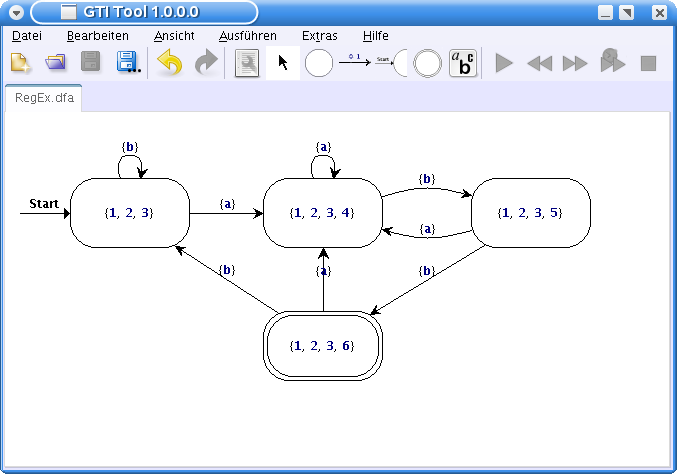
\includegraphics[width=12cm]{../images/regex_dfa.png}
\caption{Direkte Umwandlung in einen DEA}
\label{FigureRegExDFA}
\end{center}
\end{figure}
\vspace{10pt}


\section{\LaTeX-Export}

Bei der Umsetzung des \gtitools war es uns wichtig in erster Linie studentische
Benutzer zu unterstützen. Dazu zählt unter anderem das in Kapitel \ref{Print}
vorgestellte Drucken. Dadurch ist der Benutzer in der Lage seine erstellten
Automaten oder Grammatiken auszudrucken, um so seine Unterlagen zu
vervollständigen. Eine weitere wichtige Funktionen besteht in dem Bildexport.
Durch diesen Export ist der Benutzer in der Lage, die erstellten Automaten als
Bild zu exportieren, um sie zum Beispiel in eigene Ausarbeitungen
aufzunehmen.\vspace{10pt}

Als Perspektive für die Zukunft wäre es sinnvoll, auch Dozenten besser zu
unterstützen. Eine Möglichkeit wäre das Implementieren eines \LaTeX-Exports, so
dass der Lehrende nicht mehr den Umweg über den Bildexport gehen muss, sondern
den Automaten direkt in \LaTeX\ integrieren kann. Bei der Umsetzung ist auf die
Auswahl einer geeigneten Bibliothek zu achten, so dass auch große Automaten
noch gut aussehen. Wichtig wäre auch, dass sich, wenn möglich, die \LaTeX-
und die am Bildschirm dargestellte Version wenig unterscheiden.\vspace{10pt}


\section{Grammatik Erweiterungen}

Bei Grammatiken gibt es noch diverse Möglichkeiten, welche bis jetzt noch nicht
umgesetzt sind. Als Beispiele, auf die wir in diesem Kapitel noch eingehen
möchten, haben wir uns das Problem von Linksrekursion, Linksfaktorisierung und
Wortnavigation auf einer Grammatik aufgegriffen.\vspace{10pt}

\subsection{Linksrekursion}

Eine Grammatik wird als linksrekursiv bezeichnet, wenn sich aus einem beliebigen
Nichtterminalzeichen $\NonterminalSymbol{A}$ nach beliebig vielen Schritten etwas
von der Form $\NonterminalSymbol{A} \TerminalSymbol{$\alpha$}$ herleiten lässt.
Existiert eine Produktion $\NonterminalSymbol{A} \to \NonterminalSymbol{A}
\TerminalSymbol{$\alpha$}$ spricht man von direkter Rekursion. Wenn dazu mehr als
ein Ableitungsschritt nötig ist spricht man von einer indirekten
Rekursion.\vspace{10pt}

%### removes texlipse warning
In dem Buch \cite{Compilers} ist ein Algorithmus beschrieben, um Linksrekursion
bei einer Grammatik zu beseitigen, welcher sich ohne Probleme umsetzen lassen
sollte.\vspace{10pt}
%### removes texlipse warning

\noindent Gehen wir davon aus, die Produktionen für ein Nonterminal
\NonterminalSymbol{A} sind von der Form\vspace{10pt}

\NonterminalSymbol{A} $\to$ \NonterminalSymbol{A}$\alpha_1|\ldots|$
\NonterminalSymbol{A}$\alpha_n | \beta_1 | \ldots | \beta_n$\vspace{10pt}

\noindent wobei $\beta_1\ bis\ \beta_n$ nicht mit \NonterminalSymbol{A}
beginnen.\vspace{10pt}

\noindent Um diese Rekursion zu beseitigen führt man ein neues
Nichtterminalzeichen \NonterminalSymbol{A'} ein. Als ersetzt man die bestehenden Produktion von
\NonterminalSymbol{A} durch diese Produktionen:\vspace{10pt}

\NonterminalSymbol{A} $\to \beta_1 | \ldots | \beta_n$

\NonterminalSymbol{A'} $\to \alpha_1$\NonterminalSymbol{A'}$|\ldots|$
$\alpha_n$\NonterminalSymbol{A'}$|\epsilon$\vspace{10pt}

%### removes texlipse warning
\noindent Damit können wir direkte Linksrekursion beseitigen. Und dies können wir
uns auch zunutze machen, um indirekte Linksrekursion zu entfernen. Folgender
Algorithmus zur Entfernung von Linksrekursion, aus dem Buch \cite{Compilers},
macht sich dies zu nutze:\vspace{10pt}
%### removes texlipse warning

\noindent
\verb|for i = 1 to n do {|\\
\verb|  for j = 1 to i - 1 do {|\\
\verb|    ersetze jede Produktion der Form| $A_i \to A_j \gamma$ \verb| |\\ 
\verb|    durch die Produktion|$A_i \to \delta_1\gamma|\ldots|\delta_k\gamma$
\verb|, wobei |$A_j \to \delta_1|\ldots|\delta_k$\\ 
\verb|    alle derzeitigen Produktionen für |$A_j$ \verb|sind|\\ 
\verb|  }|\\
\verb|  eleminiere die unmittelbare Linksrekursion für |$A_i$\\
\verb|  (mit dem vorhergehend beschriebenen Algorithmus)|\\
\verb|}|
\vspace{10pt}

Somit besteht die Möglichkeit sowohl direkte als auch indirekte Linksrekursion
zu beseitigen.\vspace{10pt}

\subsection{Linksfaktorisierung}

Bei einer Grammatik kann es zu Problemen führen, wenn verschiedene Produktionen
gleiche Prefixe haben. Wie es zum Beispiel bei \vspace{10pt}

\noindent
$S \to$ if E then S else S
$|$ if E then S
\vspace{10pt}

\noindent
der Fall ist. Diese Probleme lassen sich durch den Algorithmus zur
Linksfaktorisierung lösen. Dieser Algorithmus sieht wie folgt aus.\vspace{10pt}

Zunächst einmal bestimmen wir eine Symbolfolge $\alpha$, welche dem längsten
gemeinsamen Prefix aller Produktionen für das selbe Nichtterminalzeichen
\NonterminalSymbol{A} entspricht. In unserem Beispiel wäre $\alpha$ "`if E then
S"'. Alle Produktionen für A sind von der Form\vspace{10pt}

\noindent
$A \to \alpha \beta_1|\ldots|\alpha
\beta_n|\gamma_1|\ldots|\gamma_n$
\vspace{10pt}

\noindent
wobei $\gamma$ nicht mit $\alpha$ beginnt und es gilt $n \geq 2$ und $k \geq 0$.
\vspace{10pt}

Um für die Grammatik den Algorithmus zur Linksfaktorisierung anzuwenden fürht
man als erstes ein neus Nichtterminalzeichen A' ein. Als
nächstes ersetzt man die bestehenden Produktionen von A
durch die folgenden.\vspace{10pt}

\noindent
$A \to \alpha A'|\gamma_1|\ldots|\gamma_n$\\
$A' \to \beta_1|\ldots|\beta_n$
\vspace{10pt}

\noindent
Dieser Schritt muss wiederholt werden, bis für kein alle Produktionen eines
Nichtterminalzeichen $\epsilon$ der einzige gemeinsame Prefix ist.\vspace{10pt} 

Dieser Algorithmus kann für eine Implementierung verwendet werden,
indem man die Bedingung für jedes Nichtterminalzeichen überprüft, ob eine Linksfatorisierung
nötig ist, und diese dann wie oben beschrieben anwendet.

\subsection{Wortnavigation für Grammatiken}

Die Wortnavigation für Automaten haben wir ja schon in Kapitel
\ref{wordNavigation} beschrieben. Solch eine Wortnavigation liese sich auch
für eine Grammatik realisieren, so dass der Benutzer nicht erst den Umweg
nutzen muss, die Grammtik in einen Autmaten umzuwandeln.\vspace{10pt}

Dabei könnte man dem Benutzer die Auswahlmöglichkeit geben, ob er via
Top-Down oder Bottom-Up Verfahren überprüfen lassen möchte, ob ein Wort in der
konstruierten Grammatik liegt. Dazu muss dann eine linksfaktorisierte Grammatik
ohne Linksrekursion verwendet werden, oder es wäre bei der Auswahl des nächsten
Schritts gegebenenfalls noch der Eingriff des Benutzers
erforderlich.\vspace{10pt}

Für die Top-Down Methode könnte das Verfahren des rekursiven Abstiegs verwendet
werden. Dieser Algorithmus startet mit dem Startsymbol der Grammatik auf dem
Keller. Wenn mehrere Produktionen für das Startsymbol in der Grammatik
existieren, muss der Benutzer jetzt auswählen, welches die richtige Produktion ist. Dann wird
das Startsymbol durch die Rechte Seite dieser Produktion ersetzt. Jetzt nimmt
man sich jedes Symbol einzeln vor wobei man von links startet. Handelt es sich
um ein Nichtterminalzeichen, würde dieses wieder durch die rechte Seite der
richtigen nächsten Produktion ersetzt. Handelt es sich um ein Terminalzeichen,
wird dieses mit dem nächsten Zeichen im Eingabewort verglichen. Wenn diese
Übereinstimmen wird ein Pointer innerhalb des Eingabewortes ein Symbol
weitergeschoben, und man betrachtet das nächste Symbol. Wenn die beiden Symbole
nicht übereinstimmen, muss eine Fehlermeldung ausgegeben werden, dass dieses
Wort mit den bis jetzt verwendeten Produktionen nich hergeleitet werden kann.
Wenn man das letzte Symbol auf dem Keller behandelt hat sollte auf dem Keller
das Eingabewort stehen. Somit kann man das Wort mit den Produktionen herleiten,
die man während dieses Durchlaufs verwendet hat. Als Hilfestellung für den
Benutzer sollten diese noch in einer Liste, oder etwas ähnlichem in der
Reihenfolge der Verwendung aufgelistet werden.\vspace{10pt}

Alternativ könnte man dem Benutzer die Möglichkeit geben ahand der Bottom-Up
Methode zu überprüfen, ob das Wort in der Grammatik liegt. Dazu wird das
komplette Eingabewort auf den Keller geschrieben. Jetzt versucht man Teile des
Kellers auf der rechten Seite einer Produktion wiederzufinden. Wenn man eine
solche Produktion gefunden hat, wird der Teil des Kellers, der der rechten
Seite entspricht, durch die linke Seite der Produktion ersetzt. Dies versucht
man fortzusetzten, bis man das Startzeichen auf dem Keller stehen hat. In
diesem Fall liegt das Eingabewort in der Grammatik. Da eventuell in einem
solchen Reduktionsschritt mehrere Produktionen in Frage kommen können, wäre
dort wieder die Entscheidung des Benutzers gefragt, welches die richtige
Produktion für diese Situation ist. Wenn keine Möglichkeit existiert das
Eingabewort auf das Startzeichen zu reduzieren, dann liegt das Wort nicht in
der konstruierten Grammatik. Wie bei der Top-Down Methode wäre es
auch hier sinnvoll, die verwendeten Produktionen in einer Liste zu
speichern, und dem Nutzer anzuzeigen, um den Vorgang nachvollziehen
zu können.\vspace{10pt}

Um auf verschiedene Benutzervorlieben einzugehen, könnte man beide Varianten
implementieren, und den Benutzer entscheiden lassen, welche er verwenden
möchte.\vspace{10pt}

\section{Erkannte Wörter ausgeben}

Eine weitere sinvolle und für die Zukunft angedachte Erweiterung ist die
Ausgabe von erkannten Wörtern. Nachdem ein Automat, eine Grammatik oder dann
vieleicht auch ein regulärer Ausdruck eingebenen und validiert wurde, soll der
Benutzer in der Lage sein eine Ansicht zu öffnen, in der er Wörter ausgegeben
bekommt, die zum Beispiel von dem erstellten Automat erkannt werden. Bei der
Umsetzung ist darauf zu achten, dass die Bestimmung dieser Wörter möglichst mit
geringer Laufzeit implementiert ist, so dass der Benutzer nicht allzu lange auf
ein Ergebnis warten muss. Die Bestimmung sollte somit nicht einfach per
Brute-Force-Methode ungesetzt werden, sondern in irgendeiner Form abhängig von
dem gewendeten Typ, wie zum Beispiel einer Grammatik. Somit sollten gewisse
Wörter direkt ausgeschlossen werden, die bei der Brute-Force-Methode ansonsten
mit getestet werden würden.\vspace{10pt}


\section{Eingabe von mehreren Wörtern}

In der aktuellen Version des \gtitools kann man nur für Automaten ein Wort
eingeben. In Zukunft soll das aber auch für Grammatiken und dann auch für
reguläre Ausdrücke möglich sein. In der aktuellen Umsetzung kann der Benutzer
aber nur ein Wort eingeben und dieses dann auf Akzeptanz prüfen. Für die
Zukunft wäre es somit wünschenswert, mehr als ein Wort eingeben zu können,
welches dann direkt während der Eingabe überprüft wird, so dass der Benutzer
nicht erst die Navigation starten muss. Diese Ansicht soll dem Benutzer helfen
zu erkennen, welche Sprache ein erstellter Automat oder eine Grammatik
erkennt.\vspace{10pt}

Eine mögliche Umsetzung wäre, dass Wörter in einer editierbaren Tabelle
eingegeben werden können. Dazu wäre in jeder Zeile ein Parser nötig, der die
Wörter erkennt. Wird eine gültige Eingabe gemacht, kann der Automat dazu
benutzt werden, dieses Wort auf Akzeptanz zu prüfen.\vspace{10pt}


\section{Benutzerinteraktion erhöhen}

Bei der Umsetzung des \gtitools war es uns sehr wichtig, dass der Benutzer
bei der Verwendung des Programms möglichst viel lernt. Im Kapitel
\ref{Concepts} wurden einige Konzepte angesprochen, die uns bei der Umsetzung
wichtig erschienen. Aufgrund des vermutlich sehr großen Aufwandes konnten wir
den Bereich Benutzerinteraktion nicht weiter ausbauen. In diesem Abschnitt
werden mögliche Anpassungen angesprochen, die für zukünftige \gtitool Versionen
geplant sind. Bei diesen Anpassungen handelt es sich zum größten Teil um
Erweiterungen der schon implementierten Umsetzungen. Alle in der Zukunft
implementierten Erweiterungen sollten dann direkt mit einer entsprechend hohen
Benutzerinteraktion umgesetzt werden, so dass das nachträgliche Erweitern in
diesen Fällen entfallen würde.\vspace{10pt}


\subsection{Word-Navigation}
Eine wichtige Erweiterung betrifft die Wort Navigation. Bei dieser Navigation
gibt es bereits eine Benutzerinteraktion, welche in \ref{InteractionPDA}
beschrieben wird. In Zukunft kann die Benutzerinteraktion, die in
\ref{wordNavigation} beschrieben wird, erweitert werden. Eine mögliche Umsetzung
wäre, den Benutzer vor einem Navigationsschritt dazu aufzufordern, die Übergänge
zu markieren, die als nächstes verwendet werden. Dabei müsste der Benutzer anhand
des nächsten Symbols im Eingabewort entscheiden, welche Übergänge dies betrifft.
Kommt ein oder mehrere $epsilon$-Übergänge vor, müssen diese Übergänge zuerst
ausgewählt werden. Durch diese Erweiterung wurde der Benutzer noch besser
erkennen können wie der Algorithmus arbeitet. Um den ungeübten Benutzer nicht zu
überfordern und somit vielleicht zur Aufgabe zu zwingen, muss dieser zusätzliche
Auswahlschritt überspringbar sein. Es muss also eine Art Raten-Funktion geben,
die dem Benutzer die Auswahl abnimmt.\vspace{10pt}


\subsection{Umwandeln}
Im Abschnitt \ref{ConverToMachine} wird das Umwandeln eines Automaten in einen
anderen Automaten beschrieben, also zum Beispiel die Umwandlung von einem
$\epsilon$-NDEA in einen DEA. Der dort Implementierte Algorithmus verwendet
verschiedene Phasen. Eine dieser Phasen ist das Bilden des
$\epsilon$-Abschlusses. In diesem Schritt wäre es möglich, den Benutzer alle
Zustände zu markieren, die von dem aktiven Zustand nur durch
$\epsilon$-Übergänge erreichbar sind.\vspace{10pt}

Eine weitere Möglichkeit wäre, den Benutzer dazu aufzufordern die Zustände zu
aktivieren, die nach einem Übergang mit einem bestimmten Symbol aktiviert sein
werden. Aber auch bei allen anderen Phasen sollte geprüft werden, ob es sinnvoll
wäre, den Benutzer zu einer Interaktion aufzufordern. Es wäre aber nicht nur
möglich Zustände und Übergänge in dem ursprünglichen Graphen zu markieren, ebenso
wäre es in dem entstehenden Graphen möglich, anzugeben, welche Zustände und
Übergänge in dem nächsten Schritt angelegt werden.\vspace{10pt}


\subsection{Erreichbare Zustände}
Wie im Abschnitt \ref{ReachableStates} vorgestellt, implementiert der
Algorithmus zur Bestimmung der erreichbaren Zustände eine Breitensuche. Bei
dieser Breitensuche könnte der Benutzer dazu aufgefordert werden die
erreichbaren Zustände zu markieren. Diese Markierung könnte dann überprüft
werden und der Benutzer würde über die Richtigkeit seiner Eingabe informiert.
Auch bei dieser Benutzerinteraktion wäre eine Funktion wichtig, die die
richtige Auswahl trifft.\vspace{10pt}


\subsection{Minimieren}
Das Minimieren von Automaten bietet sehr großen Spielraum zum Einbau von
Benutzerinteraktion. Der in Kapitel \ref{Minimize} vorgestellte Algorithmus
basiert darauf Zustände in Äquivalenz\-klassen zu unterteilen. Es wäre somit
möglich diese Unterteilung dem Benutzer zu überlassen. Er musste also
auswählen, warum eine Gruppe in zwei Gruppen zerfällt. Um dies zu erreichen,
müsste der Benutzer Übergänge mit dem gleichen Symbol finden, die in
unterschiedlichen Gruppen enden.\vspace{10pt}

Im ersten Schritt des Minimierens werden die nicht erreichbaren Zustände
entfernt, auch diesen Schritt kann der Benutzer selbst durchführen, in dem er die
entsprechenden Zustände auswählt.\vspace{10pt}


\section{Auto-Layout}\label{PerspectiveAutoLayout}

TODOBM
